
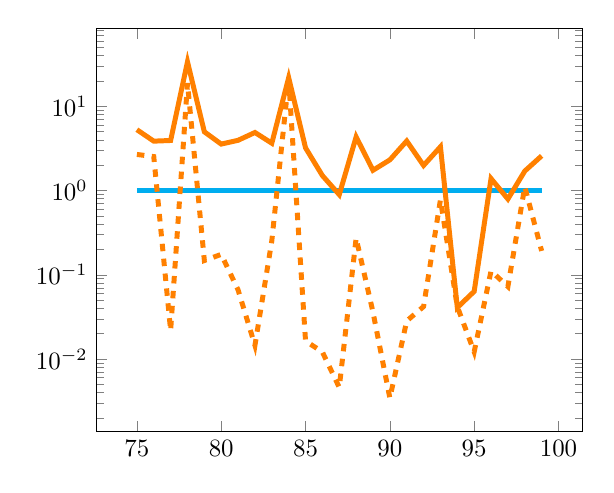
\begin{tikzpicture}[scale=0.9]
\begin{semilogyaxis}
\addplot[color=cyan,line width=2pt] coordinates {(75,1.0)(76,1.0)(77,1.0)(78,1.0)(79,1.0)(80,1.0)(81,1.0)(82,1.0)(83,1.0)(84,1.0)(85,1.0)(86,1.0)(87,1.0)(88,1.0)(89,1.0)(90,1.0)(91,1.0)(92,1.0)(93,1.0)(94,1.0)(95,1.0)(96,1.0)(97,1.0)(98,1.0)(99,1.0)};
\addplot[color=orange,line width=2pt] coordinates {(75,5.278211282898949)(76,3.8590037134609663)(77,3.93057473984575)(78,33.76203173602364)(79,4.978199248246333)(80,3.561441018868926)(81,3.950201285028903)(82,4.8899758554551696)(83,3.6479287903368993)(84,21.856756317449037)(85,3.2124334198626507)(86,1.5050589161138666)(87,0.8944976386507327)(88,4.332634508556714)(89,1.7413962718438518)(90,2.313371405039574)(91,3.8757563580002525)(92,1.9850482048793934)(93,3.310125471872353)(94,0.04082897215564973)(95,0.06350110186055002)(96,1.3870679123450598)(97,0.7932306218805735)(98,1.7028523798258246)(99,2.5806692587107003)};
\addplot[dashed,color=orange,line width=2pt] coordinates {(75,2.6818097520537236)(76,2.531284405956198)(77,0.021762499349944113)(78,18.852583182824056)(79,0.14768995464467408)(80,0.17481802080939737)(81,0.06620650448593111)(82,0.014522852016246493)(83,0.2535036946851522)(84,21.01707267443264)(85,0.01640196186918323)(86,0.012118963237737592)(87,0.004606008797724366)(88,0.2722999817632174)(89,0.03603398568549017)(90,0.003445549930269373)(91,0.028312172997047847)(92,0.04197002863349243)(93,0.7788783721741233)(94,0.04187478251225642)(95,0.012177161692412624)(96,0.11098165291960208)(97,0.07251066167828996)(98,1.1097747892946146)(99,0.19212320804849434)};

\end{semilogyaxis}
\end{tikzpicture}
